\chapter{Quick Start Example}

This chapter provides a brief introduction to Kieker based on %
a simple Bookstore application. %

Section~\ref{sec:example:downloadInstall} explains how to download and install %
Kieker. % 
The Bookstore application is introduced in Section~\ref{sec:example:bookstore}. %
The following Sections~\ref{sec:example:monitoring} %
and \ref{sec:example:analysis} demonstrate how to use \Kieker{} for monitoring %
and analyzing the monitoring data. %

% Notify-tag because this could be interesting for the reader.
\notify The presented Java sources are included in the \Kieker{} release.

\section{Download and Installation}\label{sec:example:downloadInstall}

\Kieker{} can be downloaded from \KiekerURL. The web %
site provides zip/tar.gz archives of the \Kieker{} binary distribution as well %
as the corresponding \Kieker{} source code archives.

For this chapter, it is required to download and extract an archive containing %
Kieker's binary distribution, e.g., \file{\binaryFileForDownload}.
The extracted content has the following directory structure:

\vspace{1ex}

\dirtree{%  
.1 \KiekerDir/.
.2 bin/\DTcomment{Wrapper scripts for \Kieker{} tools}. 
.3 \ldots.
.2 doc/\DTcomment{}. 
.3 tutorial/.
.4 userguide.pdf\DTcomment{PDF file of this document}.
.4 source-example/\DTcomment{Source code of the examples in this document}.
.2 dist/\DTcomment{The \Kieker{} framework libraries}.
.3 \analysisJar.
.3 \commonJar.
.3 \monitoringJar.
.3 \toolsJar.
.2 lib/\DTcomment{Libraries required by Kieker}.
.3 \ldots.
.2 META-INF/\DTcomment{Example configuration files}.
.3 \ldots.
}
% Linebreak because the text would be to close to the directory tree. 		

\section{A Simple Bookstore Application}\label{sec:example:bookstore}

The Bookstore application is a small sample application resembling a simple
bookstore where a user can search for books in an online catalog.

The following listings show the content of the source code files:

\TODO{Source code of all example classes without instrumentation}
\TODO{Ist auch die Frage, ob wir wirklich den Source-Code aller Klassen zeigen %
oder nur von den Klassen, die in Abschnitt~\ref{sec:example:monitoring} instrumentiert %
werden --- den kompletten Quelltext dann in den Anhang.}

\setJavaCodeListing
\lstinputlisting[caption=Bookstore.java]{source-example/manual-monitoring/src/mySimpleKiekerExampleManual/Bookstore.java}
\lstinputlisting[caption=CRM.java]{source-example/manual-monitoring/src/mySimpleKiekerExampleManual/CRM.java}
\lstinputlisting[caption=Catalog.java]{source-example/manual-monitoring/src/mySimpleKiekerExampleManual/Catalog.java}
\lstinputlisting[caption=BookstoreMonitoringStarter.java]{source-example/manual-monitoring/src/mySimpleKiekerExampleManual/BookstoreMonitoringStarter.java}

The example can now be compiled and executed as follows:

\setBashListing
% Note: This is different under Windows and Linux!! 		
% If the Kieker-Dir for the tutorial is changed, make sure that this is done here as well!! 		
% We cannot put a latex-macro within the listing!
\begin{lstlisting}
nils@Laptop:~/example/$ javac src/mySimpleKiekerExampleManual/*.java -d build

nils@Laptop:~/example/$ java -classpath ./build/:./lib/commons-logging-1.1.1.jar\
                        mySimpleKiekerExampleManual.BookstoreMonitoringStarter 
\end{lstlisting}

% If desired, the new created directory can be assigned to an easy remindable environment variable.
\section{Monitoring}\label{sec:example:monitoring}
For the creation of the example is is recommended to create a new working directory %
(e.g. \dir{example/}) of the following structure:

\vspace{1ex}
\dirtree{%
.1 example/. %\DTcomment{The root directory of the project}.
.2 build/\DTcomment{Directory for the Java class files}. 
.2 lib/\DTcomment{Directory for the required libraries}.
.3 \monitoringJar.
.3 \commonJar.
.3 commons-logging-1.1.1.jar.
.2 src/\DTcomment{The directory for the source code files}.
.3 mySimpleKiekerExampleManual/.
.4 Bookstore.java.
.4 BookstoreMonitoringStarter.java.
.4 Catalog.java.
.4 CRM.java.  
}
% Linebreak because the text would be to close to the directory tree. 		
\vspace{1ex}

The \Kieker{} jar-files must be copied from the \dir{\KiekerDir/dist/} directory %
of the \Kieker{} release, as described in Section~\ref{sec:example:downloadInstall}. %
The file \file{commons-logging-1.1.1.jar} is included in \dir{\KiekerDir/lib/} %
and can also be copied from there.

% The listed jar-files must be copied from the \Kieker\  directory:
% \begin{itemize}
% \item \dir{\KiekerDir/dist/\commonJar}
% \item \dir{\KiekerDir/dist/\monitoringJar}
% \item \dir{\KiekerDir/dist/commons-logging-1.1.1.jar}
% \end{itemize}

\TODO{Erz\"ahlen, was wir nun vorhaben}

\begin{figure}[H]
\begin{centering}
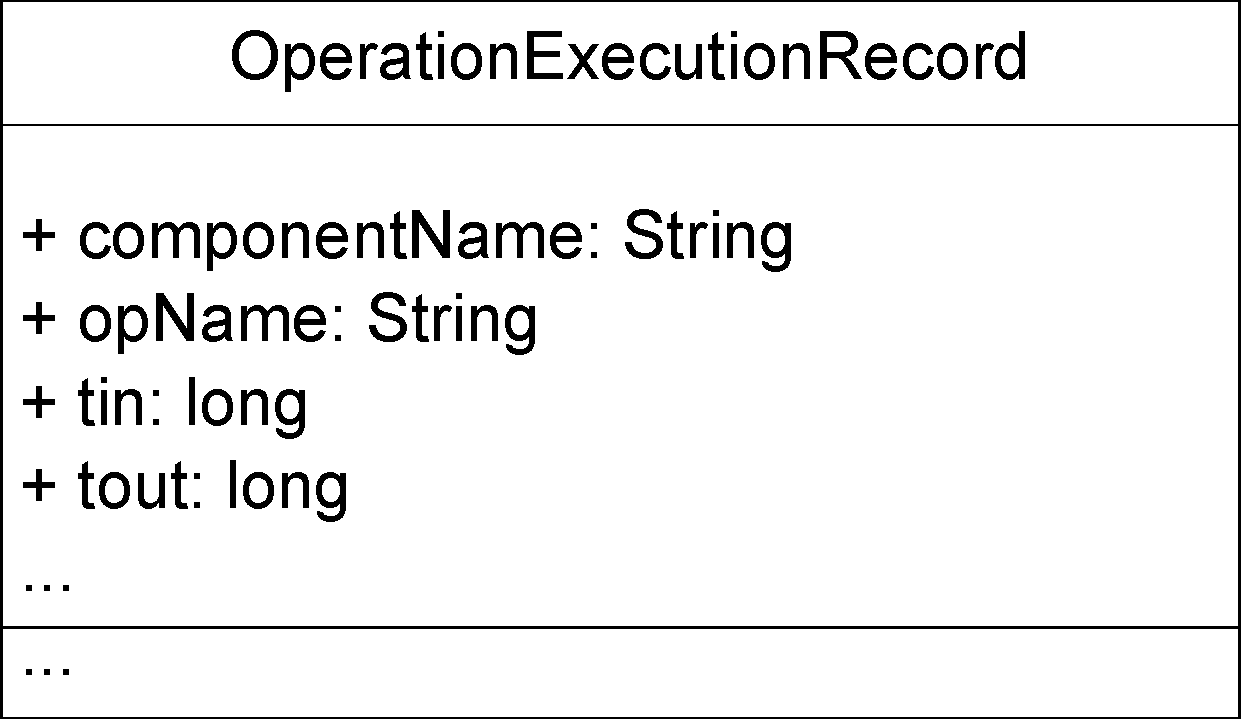
\includegraphics[width=0.4\textwidth]{images/OpExRecClassDiagram}
\caption{The class diagram of the operation execution record}
\label{Figure:OperationExecutionRecordClassDiagram}
\end{centering}
\end{figure}

The important attributes for now are:
\begin{itemize}
\item componentName: The component (the class) in which the called method is.
\item opName: The called method.
% \item traceId: The trace id of the current trace we want to record. Due to the fact, that we follow only one trace, this is zero in all recordings.
\item tin: The time before the source code which should be measured.
\item tout: The time after the source code which should be measured.
\end{itemize}

The monitoring itself is done manually. Although this is not the strength of \Kieker\ it is pretty good for a quick start. 

% Make sure that this listing will be modified, once the sourcecode changes!!!
% It must show the whole monitoring of the bookstorecall, from getting the first time to persisting of the record!!
\setJavaCodeListing
\lstinputlisting[firstline=14, lastline=29, caption=Instrumentation of the \method{getBook()} call in Bookstore.java, label=listing:cuttingBookstore]%
{source-example/manual-monitoring/src/mySimpleKiekerExampleManual/Bookstore.java}
		
In Listing \ref{listing:cuttingBookstore}  can be seen, how the monitoring itself is done. The time before and after a specific method call (in this case: \method{searchBook()}) is remembered. These information are stored in the so called operation execution record. Its (partially) layout can be seen in Figure \ref{Figure:OperationExecutionRecordClassDiagram}.

\setJavaCodeListing
\lstinputlisting[firstline=16, lastline=27, caption=Instrumentation of the \method{getBook()} call in CRM.java, label=listing:cuttingCRM]%
{source-example/manual-monitoring/src/mySimpleKiekerExampleManual/CRM.java}

The instrumented example can now be compiled and executed as follows:

\setBashListing 		
% Note: This is different under Windows and Linux!! 		
% If the Kieker-Dir for the tutorial is changed, make sure that this is done here as well!! 		
% We cannot put a latex-macro within the listing!
\begin{lstlisting}
nils@Laptop:~/example$ javac src/mySimpleKiekerExampleManual/*.java\
 -classpath ./lib/°\commonJar°:./lib/°\monitoringJar°:\
 -d build

nils@Laptop:~/example$ java\
-classpath ./build/:\
./lib/°\commonJar°:./lib/°\monitoringJar°:./lib/°\commonsLoggingJar°\
mySimpleKiekerExampleManual.BookstoreMonitoringStarter 
\end{lstlisting}
			

% warning-tag because windows has to be handled different.
\warning If the source code should be compiled and executed under Windows, the %
paths have do be seperated with semicolons instead of colons. Furthermore it is %
not possible to wrap the single parts of the commands with a backslash.\\
If everything worked correctly, there should now be a new directory with the %
name \dir{tpmon-20100727-181422131-UTC} (just with another timestamp) in the default %
temporary directory (under Linux this should be \dir{/tmp}; under Windows %
\dir{C:/temp}). In this directory, there should be a file with the extension %
\dir{.dat} which contains the recorded information from the source code and %
a file named \dir{tpmon.map} which contains information about the types of the %
monitoring records. %
The Listings~\ref{listing:exampledat} and \ref{listing:examplemap} list example %
contents. 
% A possible content of this file can be found in the appendix of this tutorial.
% We take now a closer look at the analysis.

\dirtree{%
.1 /tmp/.
.2 tpmon-20100727-181422131-UTC/.
.3 tpmon.map.
.3 tpmon-20100727-181422234-UTC-Thread-2.dat.
}

\setBashListing
\lstinputlisting[caption=tpmon-20100727-181422234-UTC-Thread-2.dat (excerpt), firstline=1, lastline=3, label=listing:exampledat]%
{ch2-quickstart-example/tpmon-20100727-181422131-UTC/tpmon-20100727-181422234-UTC-Thread-2.dat}

\lstinputlisting[caption=tpmon.map, label=listing:examplemap]%
{ch2-quickstart-example/tpmon-20100727-181422131-UTC/tpmon.map}

\section{Analysis}\label{sec:example:analysis}
As mentioned in the beginning of this chapter, it is shown how a simple consumer is programmed before starting the analysis. Therefore we need some new files:

\vspace{1ex}
\dirtree{%  
.1 example.
.2 build. 
.2 lib.
.3 \monitoringJar.
.3 \color{red}\analysisJar.
.3 \commonJar.
.3 commons-logging-1.1.1.jar.
.2 src.
.3 mySimpleKiekerExampleManual.
.4 CRM.java.  
.4 Catalog.java.
.4 Bookstore.java.
.4 BookstoreMonitoringStarter.java.
.4 \color{red}BookstoreAnalysisStarter.java.
.4 \color{red}Consumer.java.
}
\vspace{1ex}
		
The new jar-file can again be found in \dir{\KiekerDir/dist}. Listing \ref{listing:Consumer} shows the content of the new created \dir{Consumer.java}. It implements the \class{IMonitoringRecordConsumerPlugin} and overrides the necessary methods so that it can later be used by the analysis component of \Kieker. In this case the component gets a maximal response time within the constructor which will later be used to check whether a recorded method call replied fast enough or not. If the method call needed more time to response that the maximal allowed response time, it will be written directly to the error stream.\\
The methods \method{terminate} and \method{execute} don't do anything due to the fact that the consumer doesn't need any initialization. If the consumer would for example use threads then these methods would be the correct location to start and stop them.

\setJavaCodeListing       
\lstinputlisting[caption=Consumer.java, label=listing:Consumer]{source-example/manual-monitoring/src/mySimpleKiekerExampleManual/Consumer.java}

We have now to create the file \dir{BookstoreAnalysisStarter.java} to analyze our recorded information.

\setJavaCodeListing       
\lstinputlisting[caption=BookstoreAnalysisStarter.java]{source-example/manual-monitoring/src/mySimpleKiekerExampleManual/BookstoreAnalysisStarter.java}
\TODO{Dem Programm die notwendigen Dateien manuell geben.}
% notify-tag because this is a description how the analysis works.
\notify The analysis consists of the following steps:
\begin{enumerate}
\item Create a new instance (or more) of the class \class{AnalysisInstance}.
\item Register the plugins which should evaluate the records.
\item Register exactly one reader to read the stored information.
\item Start the analysis instance.
\end{enumerate}
The source code can now be executed:

\setBashListing 		
% Note: This is different under Windows and Linux!! 		
% If the Kieker-Dir for the tutorial is changed, make sure that this is done here as well!! 		
% We cannot put a latex-macro within the listing!
\begin{lstlisting}[caption=Commands to compile and run the analysis under \UnixLikeSystems{},label=lst:bookstoreAnalysisStarterLinux] 			
#\lstshellprompt{}# mkdir build
#\lstshellprompt{}# javac src/kieker/examples/userguide/ch2bookstore/manual/*.java 
        -classpath lib/#\mainJarEMF# -d build/

#\lstshellprompt{}# java -classpath build/:lib/#\mainJarEMF#
       kieker.examples.userguide.ch2bookstore.manual.BookstoreAnalysisStarter 
       /tmp/kieker-20120402-163314855-UTC-myHost-KIEKER-SINGLETON
\end{lstlisting}			

If everything worked correctly, the consumer should write something on the outputstream for every record it gets. A possible display of the run can be found in the appendix of this tutorial. 
